% Options for packages loaded elsewhere
% Options for packages loaded elsewhere
\PassOptionsToPackage{unicode}{hyperref}
\PassOptionsToPackage{hyphens}{url}
\PassOptionsToPackage{dvipsnames,svgnames,x11names}{xcolor}
%
\documentclass[
  french,
  letterpaper,
  DIV=11,
  numbers=noendperiod]{scrartcl}
\usepackage{xcolor}
\usepackage{amsmath,amssymb}
\setcounter{secnumdepth}{5}
\usepackage{iftex}
\ifPDFTeX
  \usepackage[T1]{fontenc}
  \usepackage[utf8]{inputenc}
  \usepackage{textcomp} % provide euro and other symbols
\else % if luatex or xetex
  \usepackage{unicode-math} % this also loads fontspec
  \defaultfontfeatures{Scale=MatchLowercase}
  \defaultfontfeatures[\rmfamily]{Ligatures=TeX,Scale=1}
\fi
\usepackage{lmodern}
\ifPDFTeX\else
  % xetex/luatex font selection
\fi
% Use upquote if available, for straight quotes in verbatim environments
\IfFileExists{upquote.sty}{\usepackage{upquote}}{}
\IfFileExists{microtype.sty}{% use microtype if available
  \usepackage[]{microtype}
  \UseMicrotypeSet[protrusion]{basicmath} % disable protrusion for tt fonts
}{}
\makeatletter
\@ifundefined{KOMAClassName}{% if non-KOMA class
  \IfFileExists{parskip.sty}{%
    \usepackage{parskip}
  }{% else
    \setlength{\parindent}{0pt}
    \setlength{\parskip}{6pt plus 2pt minus 1pt}}
}{% if KOMA class
  \KOMAoptions{parskip=half}}
\makeatother
% Make \paragraph and \subparagraph free-standing
\makeatletter
\ifx\paragraph\undefined\else
  \let\oldparagraph\paragraph
  \renewcommand{\paragraph}{
    \@ifstar
      \xxxParagraphStar
      \xxxParagraphNoStar
  }
  \newcommand{\xxxParagraphStar}[1]{\oldparagraph*{#1}\mbox{}}
  \newcommand{\xxxParagraphNoStar}[1]{\oldparagraph{#1}\mbox{}}
\fi
\ifx\subparagraph\undefined\else
  \let\oldsubparagraph\subparagraph
  \renewcommand{\subparagraph}{
    \@ifstar
      \xxxSubParagraphStar
      \xxxSubParagraphNoStar
  }
  \newcommand{\xxxSubParagraphStar}[1]{\oldsubparagraph*{#1}\mbox{}}
  \newcommand{\xxxSubParagraphNoStar}[1]{\oldsubparagraph{#1}\mbox{}}
\fi
\makeatother

\usepackage{color}
\usepackage{fancyvrb}
\newcommand{\VerbBar}{|}
\newcommand{\VERB}{\Verb[commandchars=\\\{\}]}
\DefineVerbatimEnvironment{Highlighting}{Verbatim}{commandchars=\\\{\}}
% Add ',fontsize=\small' for more characters per line
\usepackage{framed}
\definecolor{shadecolor}{RGB}{241,243,245}
\newenvironment{Shaded}{\begin{snugshade}}{\end{snugshade}}
\newcommand{\AlertTok}[1]{\textcolor[rgb]{0.68,0.00,0.00}{#1}}
\newcommand{\AnnotationTok}[1]{\textcolor[rgb]{0.37,0.37,0.37}{#1}}
\newcommand{\AttributeTok}[1]{\textcolor[rgb]{0.40,0.45,0.13}{#1}}
\newcommand{\BaseNTok}[1]{\textcolor[rgb]{0.68,0.00,0.00}{#1}}
\newcommand{\BuiltInTok}[1]{\textcolor[rgb]{0.00,0.23,0.31}{#1}}
\newcommand{\CharTok}[1]{\textcolor[rgb]{0.13,0.47,0.30}{#1}}
\newcommand{\CommentTok}[1]{\textcolor[rgb]{0.37,0.37,0.37}{#1}}
\newcommand{\CommentVarTok}[1]{\textcolor[rgb]{0.37,0.37,0.37}{\textit{#1}}}
\newcommand{\ConstantTok}[1]{\textcolor[rgb]{0.56,0.35,0.01}{#1}}
\newcommand{\ControlFlowTok}[1]{\textcolor[rgb]{0.00,0.23,0.31}{\textbf{#1}}}
\newcommand{\DataTypeTok}[1]{\textcolor[rgb]{0.68,0.00,0.00}{#1}}
\newcommand{\DecValTok}[1]{\textcolor[rgb]{0.68,0.00,0.00}{#1}}
\newcommand{\DocumentationTok}[1]{\textcolor[rgb]{0.37,0.37,0.37}{\textit{#1}}}
\newcommand{\ErrorTok}[1]{\textcolor[rgb]{0.68,0.00,0.00}{#1}}
\newcommand{\ExtensionTok}[1]{\textcolor[rgb]{0.00,0.23,0.31}{#1}}
\newcommand{\FloatTok}[1]{\textcolor[rgb]{0.68,0.00,0.00}{#1}}
\newcommand{\FunctionTok}[1]{\textcolor[rgb]{0.28,0.35,0.67}{#1}}
\newcommand{\ImportTok}[1]{\textcolor[rgb]{0.00,0.46,0.62}{#1}}
\newcommand{\InformationTok}[1]{\textcolor[rgb]{0.37,0.37,0.37}{#1}}
\newcommand{\KeywordTok}[1]{\textcolor[rgb]{0.00,0.23,0.31}{\textbf{#1}}}
\newcommand{\NormalTok}[1]{\textcolor[rgb]{0.00,0.23,0.31}{#1}}
\newcommand{\OperatorTok}[1]{\textcolor[rgb]{0.37,0.37,0.37}{#1}}
\newcommand{\OtherTok}[1]{\textcolor[rgb]{0.00,0.23,0.31}{#1}}
\newcommand{\PreprocessorTok}[1]{\textcolor[rgb]{0.68,0.00,0.00}{#1}}
\newcommand{\RegionMarkerTok}[1]{\textcolor[rgb]{0.00,0.23,0.31}{#1}}
\newcommand{\SpecialCharTok}[1]{\textcolor[rgb]{0.37,0.37,0.37}{#1}}
\newcommand{\SpecialStringTok}[1]{\textcolor[rgb]{0.13,0.47,0.30}{#1}}
\newcommand{\StringTok}[1]{\textcolor[rgb]{0.13,0.47,0.30}{#1}}
\newcommand{\VariableTok}[1]{\textcolor[rgb]{0.07,0.07,0.07}{#1}}
\newcommand{\VerbatimStringTok}[1]{\textcolor[rgb]{0.13,0.47,0.30}{#1}}
\newcommand{\WarningTok}[1]{\textcolor[rgb]{0.37,0.37,0.37}{\textit{#1}}}

\usepackage{longtable,booktabs,array}
\newcounter{none} % for unnumbered tables
\usepackage{calc} % for calculating minipage widths
% Correct order of tables after \paragraph or \subparagraph
\usepackage{etoolbox}
\makeatletter
\patchcmd\longtable{\par}{\if@noskipsec\mbox{}\fi\par}{}{}
\makeatother
% Allow footnotes in longtable head/foot
\IfFileExists{footnotehyper.sty}{\usepackage{footnotehyper}}{\usepackage{footnote}}
\makesavenoteenv{longtable}
\usepackage{graphicx}
\makeatletter
\newsavebox\pandoc@box
\newcommand*\pandocbounded[1]{% scales image to fit in text height/width
  \sbox\pandoc@box{#1}%
  \Gscale@div\@tempa{\textheight}{\dimexpr\ht\pandoc@box+\dp\pandoc@box\relax}%
  \Gscale@div\@tempb{\linewidth}{\wd\pandoc@box}%
  \ifdim\@tempb\p@<\@tempa\p@\let\@tempa\@tempb\fi% select the smaller of both
  \ifdim\@tempa\p@<\p@\scalebox{\@tempa}{\usebox\pandoc@box}%
  \else\usebox{\pandoc@box}%
  \fi%
}
% Set default figure placement to htbp
\def\fps@figure{htbp}
\makeatother



\ifLuaTeX
\usepackage[bidi=basic,shorthands=off]{babel}
\else
\usepackage[bidi=default,shorthands=off]{babel}
\fi
\ifLuaTeX
  \usepackage{selnolig} % disable illegal ligatures
\fi


\setlength{\emergencystretch}{3em} % prevent overfull lines

\providecommand{\tightlist}{%
  \setlength{\itemsep}{0pt}\setlength{\parskip}{0pt}}



 


\usepackage{titling}
\usepackage{graphicx}
\usepackage{setspace}

\title{Rapport du projet de traitement de données}

\pretitle{
  \begin{center}
  \large ECOLE NATIONALE DE LA STATISTIQUE ET DE L'ANALYSE DE L'INFORMATION \\ [0.5cm]
  
\includegraphics[width=4cm]{ensai.png} \\ [0.5cm]
  \normalsize PROJET TRAITEMENT DE DONNEES \\
  \textit{Etudiants 1A} \\ [1cm]
  \rule{\linewidth}{0.8pt} \\ [0.4cm]
  \LARGE \bfseries
}
\posttitle{
  \\ [0.4cm] \rule{\linewidth}{0.8pt}
  \end{center}
}

\preauthor{\begin{flushleft} \large \textit{Groupe 39 :} \\}
\postauthor{
  \begin{itemize}
    \item Gwenaël LASSALLE
    \item Théau NGUYEN-CALLOT
    \item Milyan VUKOMANOVIC
  \end{itemize}
  \end{flushleft}
}

\predate{\begin{flushright} \large \textit{Tutrice :} \\ Manon EVAIN \\ [0.2cm]}
\postdate{\end{flushright}}

\AtBeginDocument{\addtocontents{toc}{\protect\setstretch{1.5}}}
\KOMAoption{captions}{tableheading}
\makeatletter
\@ifpackageloaded{caption}{}{\usepackage{caption}}
\AtBeginDocument{%
\ifdefined\contentsname
  \renewcommand*\contentsname{Table des matières}
\else
  \newcommand\contentsname{Table des matières}
\fi
\ifdefined\listfigurename
  \renewcommand*\listfigurename{Liste des Figures}
\else
  \newcommand\listfigurename{Liste des Figures}
\fi
\ifdefined\listtablename
  \renewcommand*\listtablename{Liste des Tables}
\else
  \newcommand\listtablename{Liste des Tables}
\fi
\ifdefined\figurename
  \renewcommand*\figurename{Figure}
\else
  \newcommand\figurename{Figure}
\fi
\ifdefined\tablename
  \renewcommand*\tablename{Table}
\else
  \newcommand\tablename{Table}
\fi
}
\@ifpackageloaded{float}{}{\usepackage{float}}
\floatstyle{ruled}
\@ifundefined{c@chapter}{\newfloat{codelisting}{h}{lop}}{\newfloat{codelisting}{h}{lop}[chapter]}
\floatname{codelisting}{Listing}
\newcommand*\listoflistings{\listof{codelisting}{Liste des Listings}}
\makeatother
\makeatletter
\makeatother
\makeatletter
\@ifpackageloaded{caption}{}{\usepackage{caption}}
\@ifpackageloaded{subcaption}{}{\usepackage{subcaption}}
\makeatother
\usepackage{bookmark}
\IfFileExists{xurl.sty}{\usepackage{xurl}}{} % add URL line breaks if available
\urlstyle{same}
\hypersetup{
  pdflang={fr},
  colorlinks=true,
  linkcolor={black},
  filecolor={Maroon},
  citecolor={Blue},
  urlcolor={Blue},
  pdfcreator={LaTeX via pandoc}}


\author{}
\date{}
\begin{document}


\maketitle
\thispagestyle{empty}
\newpage

\setcounter{page}{1}

\renewcommand{\contentsname}{Sommaire}

\tableofcontents

\newpage

\section*{Introduction}\label{introduction}
\addcontentsline{toc}{section}{Introduction}

Le domaine du sport de haut niveau a connu, au cours de la dernière
décennie, une révolution majeure. Qu'il s'agisse de l'optimisation des
performances des athlètes, de l'analyse tactique ou de l'engagement des
passionnés, la donnée est devenue un pilier central de l'écosystème
sportif mondial. Cependant, la variété de disciplines allant des sports
de ballon collectifs aux sports de raquette individuels pose un défi
informatique de taille : comment concevoir un système capable d'unifier
et de traiter des données aux structures hétérogènes ?

Dans le cadre de ce projet de traitement de données, nous avons
développé « TGM Statistiques », une plateforme logicielle conçue pour
centraliser et analyser les statistiques de deux disciplines majeures :
le basketball et le tennis. Se concentrer sur seulement deux sports est
un choix fort : cela nous permet de privilégier la profondeur d'analyse
à la quantité. En proposant des indicateurs très détaillés sur le
déroulé précis des rencontres, à l'instar d'applications de référence
comme Flashscore, notre outil offre une exploitation fine des données,
utile tant pour les analystes techniques que pour les passionnés de
sport. L'objectif de ce projet n'est pas seulement de fournir des
indicateurs de performance, mais de proposer une architecture logicielle
robuste et générique, fondée sur les principes de la programmation
orientée objet.

Notre démarche s'articule autour de trois axes principaux présentés dans
ce rapport. Dans un premier temps, nous décrivons les jeux de données
utilisés et les méthodes d'ingestion flexibles que nous avons mises en
place pour pallier la diversité des formats CSV. Ensuite, nous exposons
la modélisation logicielle à travers nos diagrammes de classes UML,
justifiant nos choix de conception pour garantir l'extensibilité du
programme. Enfin, nous présentons les fonctionnalités de notre interface
de consultation, permettant d'explorer les historiques de matchs et les
classements de manière interactive.

\newpage

\section{Présentation du projet}\label{pruxe9sentation-du-projet}

\subsection{Contexte}\label{contexte}

Le présent projet s'inscrit dans le cadre du Projet de Traitement de
Données. Le cahier des charges initial nous imposait de concevoir une
application Python respectant les principes fondamentaux de la
Programmation Orientée Objet, avec une contrainte de généralisabilité
absolue. Le code devait être capable de traiter des jeux de données
variés, permettant ainsi une grande adaptabilité. Le but de notre
application est donc de proposer un système faisant abstraction des
règles spécifiques à chaque sport pour offrir un outil d'analyse
statistique universel. À travers ce projet, nous avons voulu démontrer
qu'une modélisation logicielle rigoureuse permet de transformer des
fichiers CSV diverses en une source d'information cohérente, permettant
de consulter des classements et des historiques de performances sur
quelques disciplines.

\subsection{Besoins fonctionnels}\label{besoins-fonctionnels}

L'application a pour mission principale de centraliser et de transformer
des données sportives brutes en informations exploitables pour
l'utilisateur. Pour cela, elle doit répondre en premier lieu à un besoin
d'importation et de normalisation, capable de lire différents flux de
données tout en nettoyant les éventuelles erreurs ou informations
manquantes pour garantir une base de travail fiable. Une fois ces
données intégrées, le système assure le calcul automatique de
statistiques personnalisées, allant des bilans classiques de victoires
et de défaites aux indicateurs de performance plus techniques et
spécifiques à la discipline concernée. L'accès à ces informations est
ensuite facilité par une interface de consultation intuitive qui permet
à l'utilisateur de naviguer dans les données, d'effectuer des recherches
ciblées sur des joueurs ou des équipes, de filtrer les résultats selon
divers critères et de consulter des historiques complets.

\subsection{Présentation des
données}\label{pruxe9sentation-des-donnuxe9es}

Nous avons choisi d'utiliser seulement certains jeux de données parmi
ceux proposés afin de modéliser notre application. Notre sélection a été
pensée pour diversifier au maximum notre approche : nous avons ainsi
veillé à inclure à la fois un sport collectif et un sport individuel,
tout en intégrant des données issues à la fois du sport masculin et du
sport féminin. Dans cette optique, nous avons travaillé à partir des
fichiers suivants :

\begin{itemize}
\tightlist
\item
  \textbf{Basket-ball} :

  \begin{itemize}
  \tightlist
  \item
    \texttt{game.csv} : Données sur les matchs NBA.
  \item
    \texttt{player.csv} : Informations sur les joueurs NBA.
  \item
    \texttt{team.csv} : Informations sur les équipes NBA.
  \end{itemize}
\item
  \textbf{Tennis} :

  \begin{itemize}
  \tightlist
  \item
    \texttt{atp\_matches\_2024.csv} : Résultats détaillés des matchs du
    circuit ATP.
  \item
    \texttt{atp\_players\_2024.csv} : Informations sur les joueurs du
    circuit ATP.
  \item
    \texttt{wta\_matches\_2024.csv} : Résultats détaillés des matchs du
    circuit WTA.
  \item
    \texttt{wta\_players\_2024.csv} : Informations sur les joueuses du
    circuit WTA.
  \end{itemize}
\end{itemize}

Le choix du basket-ball et du tennis s'appuie sur la richesse et la
précision des données statistiques qu'ils génèrent, offrant une analyse
bien plus fine que le simple score final. Par exemple, au basket-ball,
il est possible d'évaluer les pourcentages de réussite aux tirs, que ce
soit à l'échelle collective ou individuelle. De la même manière, le
tennis offre des indicateurs techniques cruciaux tels que le nombre
d'aces, de doubles fautes ou d'erreurs directes. L'exploitation de ces
statistiques avancées permet de dépasser le résultat brut pour
comprendre le déroulement réel du match. Cette approche est
particulièrement pertinente pour les analystes souhaitant s'appuyer sur
des données détaillées afin de comprendre les tendances de jeu et
d'anticiper les performances lors de rencontres futures.

Avant de débuter l'analyse de nos différents jeux de données sportives,
nous avons réalisé une phase d'exploration approfondie afin d'en
garantir la fiabilité. Cette étape a consisté à identifier d'éventuels
doublons et à recenser les valeurs manquantes qui auraient pu provoquer
des erreurs lors de certaines demandes. Ces vérifications préliminaires
nous permettent de confirmer que les bases de données sont exploitables.

\section{Conception de l'application}\label{conception-de-lapplication}

\subsection{Modélisation}\label{moduxe9lisation}

\begin{figure}[H]

{\centering 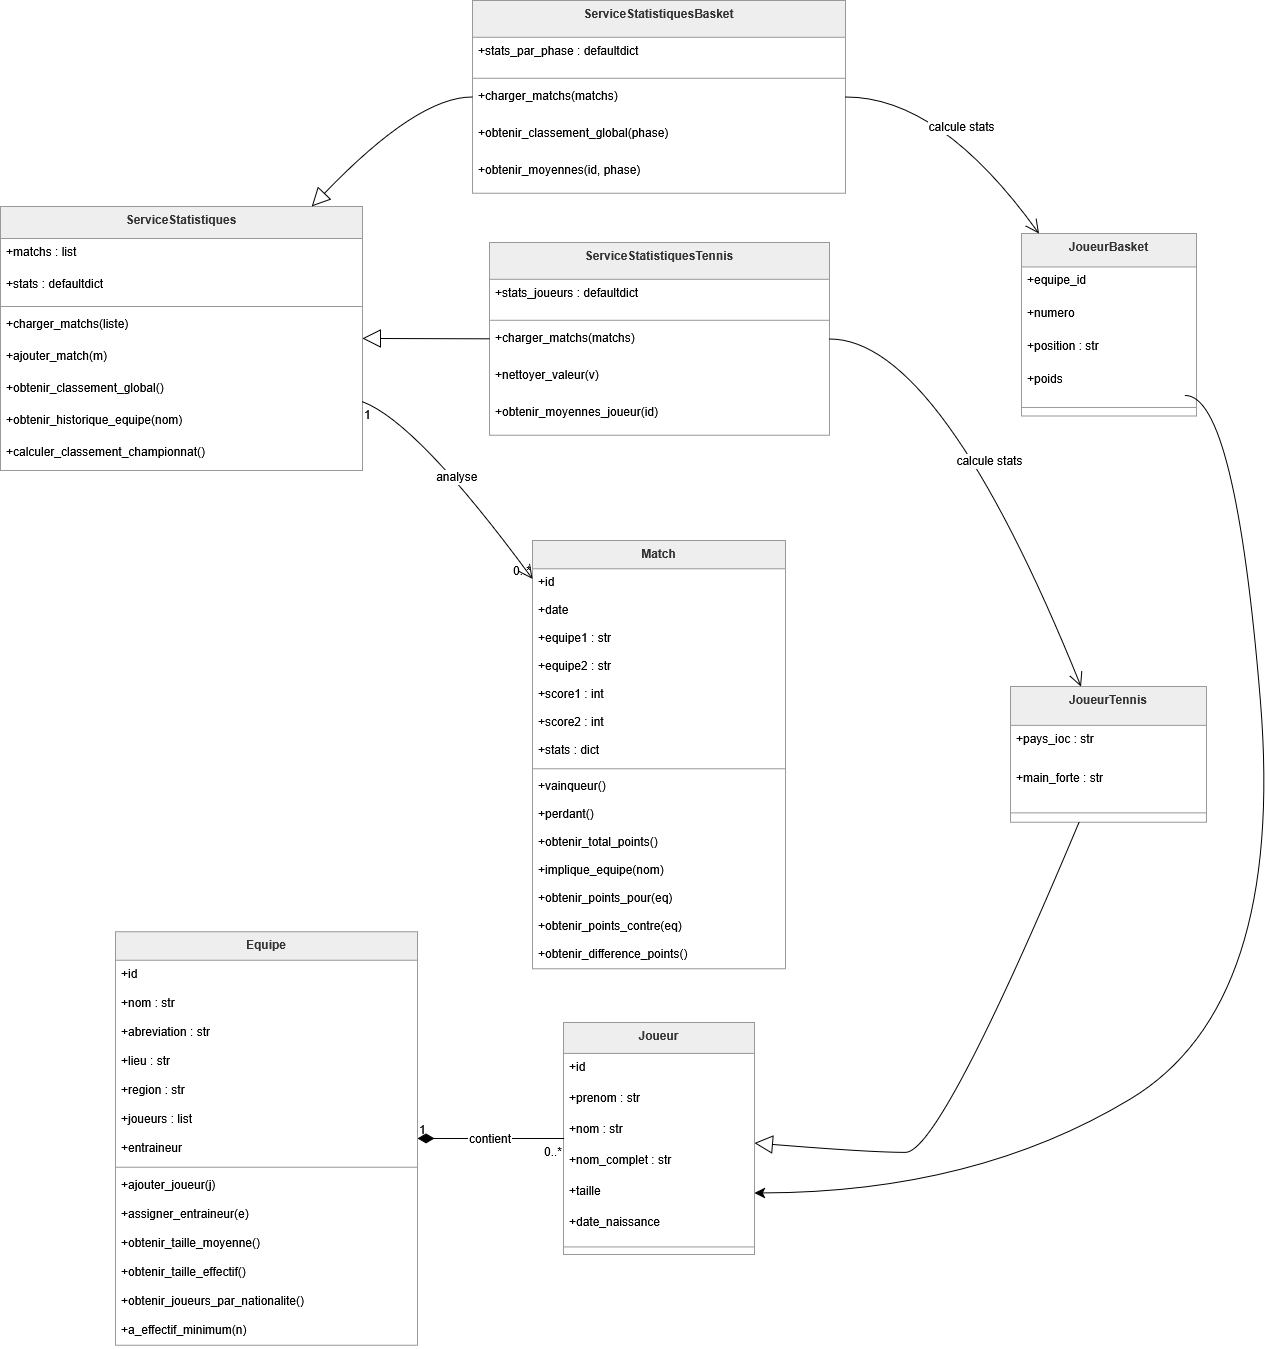
\includegraphics[width=1\linewidth,height=\textheight,keepaspectratio]{images/Diagramme_de_classe.png}

}

\caption{Diagramme de classe}

\end{figure}%

Le projet est structuré autour de plusieurs classes regroupées dans le
package pkg. La couche models constitue le noyau de notre projet : la
classe Joueur et ses spécialisations JoueurBasket et JoueurTennis, la
classe Match avec son dictionnaire stats générique, et la classe Equipe
qui agrège un effectif de joueurs toutes représentées dans le diagramme
ci-dessus. La couche adapter assure la conversion des données brutes CSV
en objets Python directement manipulables. La classe abstraite
BaseAdapter impose le fonctionnement via les méthodes adapt() et
to\_row(), dont héritent BasketJoueurAdapter et TennisJoueurAdapter pour
les joueurs, ainsi que leurs équivalents pour les matchs. Ce découpage
permet d'absorber les différences de format entre les datasets NBA et
Tennis sans impacter le reste du code. La couche repository s'appuie sur
DataRepository, qui orchestre le chargement et la sauvegarde des
fichiers CSV en déléguant la conversion à l'adaptateur correspondant. La
couche services porte l'intelligence de l'application.
ServiceAnnuaireJoueurs gère les profils et expose des filtres par équipe
ou par pays. ServiceStatistiques, ServiceStatistiquesBasket et
ServiceStatistiquesTennis représentées dans le diagramme prennent en
charge les classements et moyennes. Enfin, ServiceApplication orchestre
la navigation de l'interface console en s'appuyant sur l'ensemble de ces
services.

\begin{figure}[H]

{\centering 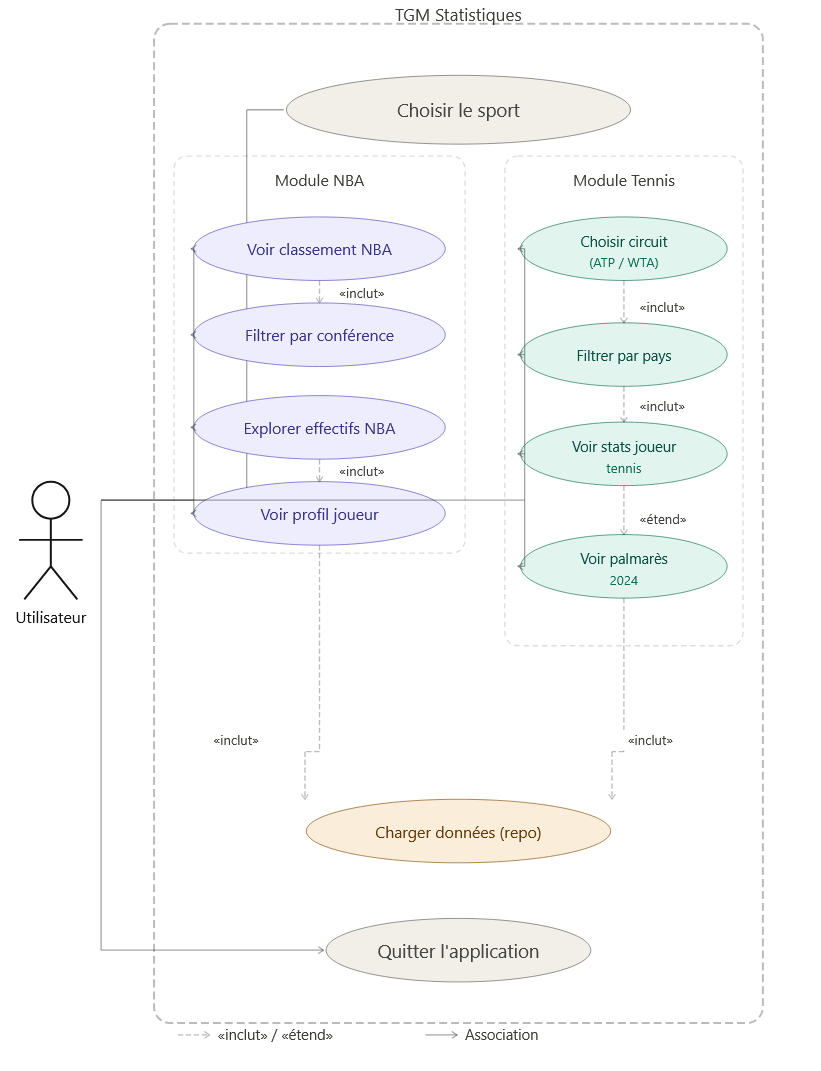
\includegraphics[width=1\linewidth,height=\textheight,keepaspectratio]{images/diagramme_cas_utilisation.png}

}

\caption{Diagramme de cas d'utilisation}

\end{figure}%

Le diagramme de cas d'utilisation de notre application fait apparaître
un unique acteur l'Utilisateur qui interagit avec l'ensemble du système
via un menu console. Au lancement, l'utilisateur choisit un sport. S'il
sélectionne le module NBA, un sous-menu lui propose deux options. La
première lui permet de consulter le classement et les statistiques
avancées des équipes : il choisit d'abord une phase (Saison Régulière ou
Playoffs), puis une conférence (Est, Ouest ou Global). L'application
charge alors les matchs via DataRepository, calcule les victoires et les
moyennes par équipe (points marqués et encaissés, rebonds, passes,
interceptions, contres, pourcentages de tir) et affiche le classement
filtré. La seconde option lui permet d'explorer les effectifs : il
sélectionne une équipe parmi la liste organisée par conférence, consulte
son effectif trié par numéro de maillot, puis choisit un joueur pour
accéder à sa carte détaillée (position, taille, poids, date de
naissance). S'il sélectionne le module Tennis, un sous-menu lui propose
de choisir entre le circuit ATP et le circuit WTA. Dans les deux cas, le
déroulé est identique : l'application affiche les codes pays
disponibles, ce qui nécessite de connaître le pays du joueur que l'on
recherche, ce qui peut être contraignant. Toutefois c'est la méthode qui
nous paraissait être la plus pertinente pour avoir accès à un maximum de
joueurs. L'utilisateur saisit donc un pays, puis choisit un joueur parmi
ceux représentant le pays choisi. Il accède alors à la fiche complète du
joueur, comprenant ses statistiques agrégées sur la saison (victoires,
défaites, aces par match, double-fautes, temps de jeu moyen, balles de
break sauvées et converties) ainsi que son palmarès des tournois
remportés en 2024. Enfin Quitter l'application est accessible à tout
moment depuis le menu principal

\newpage

\subsection{Architecture générale}\label{architecture-guxe9nuxe9rale}

Notre projet repose sur une structure orientée objet qui privilégie la
modularité et l'organisation. L'architecture repose sur plusieurs
modules, chacun ayant une responsabilité bien définie :

\begin{Shaded}
\begin{Highlighting}[]

\NormalTok{projet/}
\NormalTok{├── main.py}
\NormalTok{├── pyproject.toml}
\NormalTok{├── README.md}
\NormalTok{└── pkg/}
\NormalTok{    ├── \_\_init\_\_.py}
\NormalTok{    ├── models/}
\NormalTok{    │   ├── \_\_init\_\_.py}
\NormalTok{    │   ├── joueur.py}
\NormalTok{    │   ├── equipe.py}
\NormalTok{    │   └── match.py}
\NormalTok{    ├── adapter/}
\NormalTok{    │   ├── \_\_init\_\_.py}
\NormalTok{    │   ├── base\_adapter.py}
\NormalTok{    │   ├── generic\_joueur\_adapter.py}
\NormalTok{    │   ├── generic\_equipe\_adapter.py}
\NormalTok{    │   └── generic\_match\_adapter.py}
\NormalTok{    ├── repository/}
\NormalTok{    │   ├── \_\_init\_\_.py}
\NormalTok{    │   └── data\_repository.py}
\NormalTok{    ├── config/}
\NormalTok{    │   ├── \_\_init\_\_.py}
\NormalTok{    │   └── dataset\_configuration.py}
\NormalTok{    ├── services/}
\NormalTok{    │   ├── \_\_init\_\_.py}
\NormalTok{    │   ├── service\_application.py}
\NormalTok{    │   ├── service\_statistiques.py}
\NormalTok{    │   ├── service\_annuaire\_joueur.py}
\NormalTok{    │   └── services\_matchs.py}
\NormalTok{    └── tests/}
\NormalTok{        ├── \_\_init\_\_.py}
\NormalTok{        ├── test\_models.py}
\NormalTok{        ├── test\_adapters.py}
\NormalTok{        ├── test\_services.py}
\NormalTok{        └── test\_repository.py}
\end{Highlighting}
\end{Shaded}

(bien expliquer la logique de cette architecture car bcp de points sur
le rapport)

\subsection{Choix technologiques}\label{choix-technologiques}

Le choix de Python 3.12 associé à une architecture
Repository/Adapter/Service et à la Programmation Orientée Objet permet
de construire une application modulaire, où les classes abstraites
facilitent l'intégration de nouvelles sources de données sportives sans
fragiliser le système. La bibliothèque \emph{Pandas} est ici
indispensable pour manipuler les fichiers CSV : elle transforme les
données brutes en DataFrames pour permettre un filtrage, un tri et une
organisation ultra-rapide des performances. Pour la partie analytique,
le module math assure la précision des calculs techniques complexes
tandis que l'outil \emph{defaultdict} du module collections simplifie la
création de dictionnaires de statistiques en gérant automatiquement
l'initialisation des scores pour chaque nouveau joueur ou équipe. Enfin,
la fiabilité du code est garantie par \emph{pytest} et
\emph{unittest.mock} : les MagicMock agissent comme des ``doublures''
qui imitent des fichiers, tandis que les patches détournent les appels
du programme vers ces faux composants plutôt que vers le disque dur.
Concrètement, cela permet de faire croire au programme qu'il lit un
fichier réel pour vérifier instantanément s'il calcule bien les
classements, même dans des cas compliqués ou face à des erreurs (comme
un fichier corrompu), sans avoir besoin de créer ou de manipuler de
vrais documents sur l'ordinateur.

\section{Réalisation}\label{ruxe9alisation}

\subsection{Organisation du travail}\label{organisation-du-travail}

L'organisation de ce projet a débuté par une phase de réflexion
collective afin de structurer les axes majeurs de développement de
l'application. Cette première étape de modélisation nous a permis
d'accorder nos visions techniques avant que l'arrivée concrète des jeux
de données ne nous permette d'affiner la structure des classes et la
logique des méthodes de traitement.

Une fois ce cadre méthodologique établi, nous avons réparti le
développement technique de la façon suivante : Théau s'est occupé de la
gestion du flux de données, développant les scripts d'insertion et les
adaptateurs nécessaires à l'intégration, tandis que Milyan s'est
concentré sur l'architecture logicielle en codant l'ensemble des classes
structurantes du système. En parallèle, Gwenaël a pris en charge le
contrôle qualité à travers la vérification de la propreté des données,
tout en concevant l'interface utilisateur afin de permettre une
accessibilité simple aux données.

Parallèlement au développement, nous avons mis en place une stratégie de
tests modulaires pour garantir la fiabilité de chaque couche de notre
application. Théau a pris en charge la validation des flux d'entrée via
les tests d'adaptateurs (\emph{test\_adapters.py}), Milyan a assuré la
conformité des entités métier à travers les tests de modèles
(\emph{test\_models.py}), tandis que Gwenaël s'est occupé de valider la
logique globale et les calculs statistiques dans les tests de services
(\emph{test\_services.py}).

Afin de fluidifier notre collaboration et d'assurer la cohérence de
notre développement, nous avons utilisé Git. Cet outil a été
indispensable pour travailler simultanément sur le même code source,
gérer les fusions de nos travaux respectifs et conserver un historique
rigoureux de chaque étape du projet.

Nous avons ensuite rédigé le rapport tous les trois, en choisissant
d'utiliser l'outil Quarto.

\subsection{Développement}\label{duxe9veloppement}

\subsection{Difficultés
rencontrées}\label{difficultuxe9s-rencontruxe9es}

L'une des principales difficultés de ce projet a résidé dans son
démarrage : en l'absence de sujet imposé et n'ayant pas encore les jeux
de données à notre disposition, il a été particulièrement complexe de
lancer une dynamique de travail concrète. Cette phase d'incertitude a
rendu difficile la définition du concept même de notre future
application, car il est délicat de structurer une architecture
logicielle ou d'imaginer des fonctionnalités pertinentes sans connaître
la nature exacte, le volume et les contraintes des données à traiter.

La gestion de l'héritage et des classes abstraites a représenté un défi
structurel majeur, notamment pour concevoir une hiérarchie cohérente
entre les joueurs et les adaptateurs spécifiques au basketball et au
tennis. Pour résoudre cette difficulté, nous avons mené une réflexion
approfondie afin de bien identifier les attributs communs et les besoins
spécifiques à chaque sport, ce qui a permis d'implémenter une structure
solide évitant toute duplication de code.

Le traitement des données « sales » dans les fichiers CSV réels, comme
les valeurs manquantes ou les formats incohérents, a nécessité une
attention particulière. Nous avons résolu ce problème en intégrant des
mécanismes de nettoyage et de conversion directement dans les classes
\emph{StatistiqueJoueur} et \emph{ServiceAnnuaireJoueurs}, assurant la
transformation systématique des données (conversion en float ou passage
des lbs aux kg) et le filtrage des valeurs inexploitables.

La séparation des responsabilités entre les différents services
(Statistiques, Annuaire, Matchs) est devenue de plus en plus délicate à
mesure que la taille du projet augmentait. Pour éviter que leurs
fonctions ne se chevauchent, nous avons mené un exercice d'architecture
logicielle rigoureux, redéfinissant précisément le rôle de chaque
service pour garantir que chaque composant ne s'occupe que de sa mission
spécifique.

Enfin, le couplage entre les adaptateurs et les modèles de données
présentait une fragilité : le moindre changement dans un nom de colonne
CSV pouvait bloquer l'application. Nous avons stabilisé ce point en
utilisant des valeurs par défaut lors de la récupération des données
(via la méthode row.get(col, ``N/A'')), apportant ainsi la rigueur
nécessaire pour que le programme reste fonctionnel et robuste même en
cas de données manquantes ou de modifications imprévues des fichiers
sources.

\newpage

\section{Tests et validation}\label{tests-et-validation}

\subsection{Stratégie de test}\label{stratuxe9gie-de-test}

Pour garantir la fiabilité de notre application, nous avons mis en place
une stratégie de tests unitaires et d'intégration basée sur le framework
Pytest. L'objectif est double : assurer l'exactitude des calculs
statistiques et garantir la robustesse des processus d'importation.

La validation commence avec les modèles et les adaptateurs. Les tests
sur les modèles garantissent que chaque objet métier, comme un match ou
un joueur, est instancié avec des données saines et que ses propriétés
calculées (par exemple, la concaténation du nom complet) se comportent
de manière prévisible. Parallèlement, la couche des adaptateurs fait
l'objet d'une attention critique. Nous y testons le mapping entre le
format brut des dictionnaires issus du CSV et nos objets Python, en
mettant à l'épreuve la gestion des valeurs manquantes et la précision
des conversions techniques, telles que la transformation des poids de
lbs en kg.

Le cœur du programme, regroupé dans la partie services, est quant à lui
vérifié par des tests précis sur les calculs et les règles de gestion.
Ces tests permettent de contrôler que les classements des équipes, les
moyennes de points ou encore l'historique des joueurs sont calculés sans
aucune erreur. Pour que ces vérifications soient fiables et rapides,
nous utilisons des simulations (appelées ``Mocks'') qui remplacent les
fichiers réels par des données fictives mais contrôlées. Cela nous
permet de tester le ``cerveau'' de l'application de façon isolée, en
étant certains que si un résultat est faux, cela vient d'une erreur de
calcul et non d'un problème technique lié au chargement des données.

Enfin, la fiabilité de la persistance et de l'accès aux données est
assurée par des tests aux frontières au niveau des repositories et des
importeurs. Nous utilisons des environnements de fichiers temporaires
via \emph{tmp\_path}. Cette méthode nous permet de vérifier, dans des
conditions quasi réelles, que le système gère correctement les
différents séparateurs et l'encodage des fichiers CSV. Cette stratégie
globale assure ainsi une interface fluide et sécurisée entre le stockage
physique et la logique métier de l'application.

\newpage

\subsection{Quelques résultats}\label{quelques-ruxe9sultats}

!
\includegraphics[width=\linewidth,height=10cm,keepaspectratio,alt={Légende de l'image}]{~/Projet_TDD/projetTDD_2026_structure/Projet_Tdd/images/1er_menu.png}

!
\includegraphics[width=\linewidth,height=10cm,keepaspectratio,alt={Légende de l'image}]{~/Projet_TDD/projetTDD_2026_structure/Projet_Tdd/images/1er_menu_tennis.png}

\begin{figure}[H]

{\centering 
\includegraphics[width=\linewidth,height=10cm,keepaspectratio]{~/Projet_TDD/projetTDD_2026_structure/Projet_Tdd/images/cover_tests.png}

}

\caption{Légende de l'image}

\end{figure}%

\begin{figure}[H]

{\centering 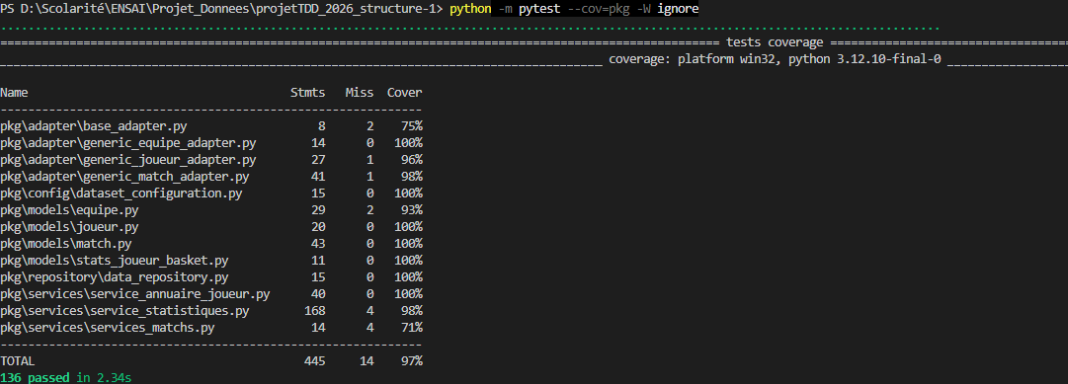
\includegraphics[width=1\linewidth,height=\textheight,keepaspectratio]{images/cover_tests.png}

}

\caption{Légende de l'image}

\end{figure}%

\subsection{Limites de l'application}\label{limites-de-lapplication}

Le choix de nous concentrer exclusivement sur deux sports rend
l'application particulièrement spécifique. L'interface utilisateur ayant
été finement adaptée aux caractéristiques propres de ces disciplines,
cette spécialisation crée une contrainte majeure en termes d'évolutivité
: l'ajout d'un nouveau sport s'avère complexe. En effet, chaque nouvelle
catégorie nécessiterait une adaptation de l'interface pour répondre à
ses spécificités, ce qui limite sa capacité à s'ouvrir à d'autres
domaines sportifs sans un travail de développement supplémentaire
conséquent.

\newpage

\section*{Conclusion}\label{conclusion}
\addcontentsline{toc}{section}{Conclusion}

\newpage

\section*{Annexes}\label{annexes}
\addcontentsline{toc}{section}{Annexes}

!
\includegraphics[width=\linewidth,height=10cm,keepaspectratio,alt={Légende de l'image}]{~/Projet_TDD/projetTDD_2026_structure/Projet_Tdd/images/1er_menu_NBA.png}

!
\includegraphics[width=\linewidth,height=10cm,keepaspectratio,alt={Légende de l'image}]{~/Projet_TDD/projetTDD_2026_structure/Projet_Tdd/images/Annuaire_des_equipes.png}

!
\includegraphics[width=\linewidth,height=10cm,keepaspectratio,alt={Légende de l'image}]{~/Projet_TDD/projetTDD_2026_structure/Projet_Tdd/images/carte_d_un_joueur.png}




\end{document}
